\documentclass[12pt]{article}
\usepackage[T2A]{fontenc}
\usepackage[utf8]{inputenc}
\usepackage[russian]{babel}
\usepackage[a4paper,left=2.5cm, right=1.5cm, top=2.5cm, bottom=2.5cm]{geometry}
\usepackage{graphicx}

\begin{document}
\title{Моделирование подразделений МЧС на основе
групповых объектов}

\author{Ю.В. Седельников}
\date{\today}
\maketitle

\abstract
В настоящее время для управления процессом ликвидации последствий чрезвычайных
ситуаций широко используются системы поддержки принятия решений на основе
имитационного моделирования. Такие системы представляют собой специализированные
приложения, которые позволяют работать с цифровыми картами местности путем нанесения
обстановки, проведения расчетов, манипулирования объектами.

\section{Текст}

Одной из задач при построении моделей подобных
систем является создание моделей подразделений
МЧС. Особенности функционирования таких подразделений дают возможность представить их в виде групповых объектов.
В общем случае с помощью группового объекта
можно представить имитационную модель некоторой
системы, состоящую из элементов и связей между ними, функционирующих в определенные дискреты времени. Например, на его основе можно представить пожарный расчет, войска ГО, поисково-спасательную
службу и т. д.
При построении СППР ликвидации последствий
чрезвычайных ситуаций необходимо разработать следующие модели подразделений МЧС (рис. 1).
Моделируемые подразделения МЧС имеют следующую структуру.
Поисково-спасательная служба — это подразделения, которые должны выполнять функции по проведению поисково-спасательных операций в зоне ЧС.
В СППР ее можно представить в виде информационной модели (рис. 2).
Войска ГО должны обеспечивать функции эвакуации и поддержания жизнеобеспечения населения, восстановления поврежденных объектов и коммуникаций.
Их информационная модель в СППР представлена
на рис. 3.
Пожарная охрана должна выполнять функции тушения пожаров и проведения первоочередных аварийноспасательных операций. На рис. 4 представлена ее информационная модель в СППР.
Психологическая служба должна обеспечивать
функции оказания экстренной психологической помощи пострадавшим. Ее модель представлена
на рис. 5.
«Центроспас» должен выполнять функции оперативного реагирования при возникновении ЧС, модель которых приведена на рис. 6.

\center{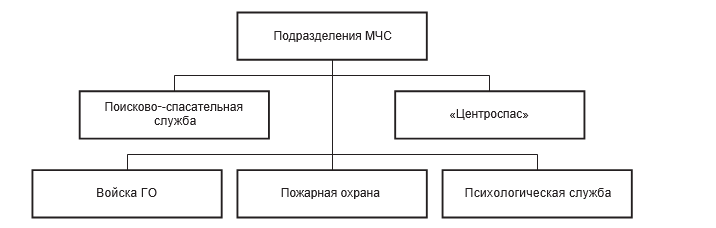
\includegraphics[scale=0.5]{1.png}}

\begin{itemize}
\item набирать текст;
\item управлять начертанием и размером шрифта;
\item а теперь ещё и создали список.
\end{itemize}

\section{Немного математики}

Формулу можно поместить внутрь текста: \( y=\sin x \) или сделать отдельным абзацем:

\[
\int_a^b x^2 dx = \left. \frac{x^3}{3} \right|_a^b .
\]

\section{Иллюстрации}

Вставим рисунок и сошлёмся на него (рис.~\ref{lion})

\begin{figure}[h]
\center{
\includegraphics[scale=0.5]{TeX_lion.jpg}}
\caption{Талисман \TeX, созданный художником Дуэйном Бибби}
\label{lion}
\end{figure}

\end{document}